\documentclass[tikz,border=8pt]{standalone}
\usepackage{tikz}
\usetikzlibrary{positioning,arrows.meta,calc}
\begin{document}
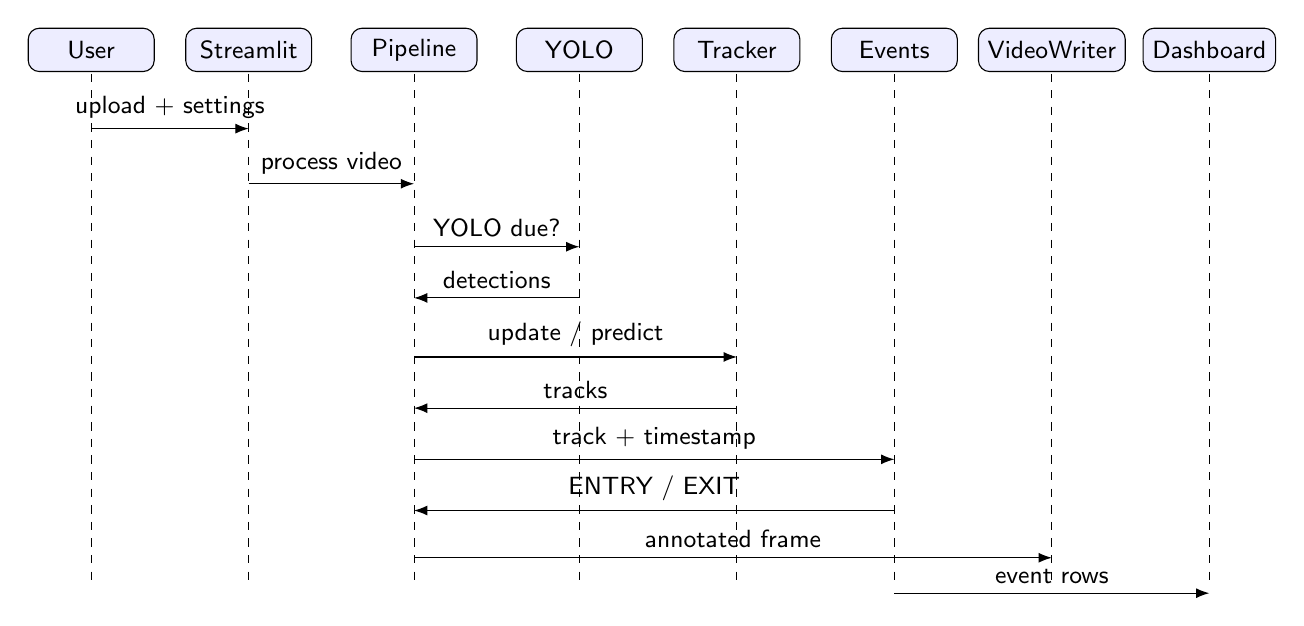
\begin{tikzpicture}[font=\sffamily\small, >=Latex]
  \def\xU{0} \def\xUI{2.0} \def\xP{4.1} \def\xY{6.2} \def\xT{8.2} \def\xE{10.2} \def\xV{12.2} \def\xD{14.2}
  \foreach \x/\name in {\xU/User,\xUI/Streamlit,\xP/Pipeline,\xY/YOLO,\xT/Tracker,\xE/Events,\xV/VideoWriter,\xD/Dashboard}{
    \node[draw,rounded corners,fill=blue!7,minimum width=1.6cm,minimum height=0.55cm] at (\x,0) {\name};
    \draw[dashed] (\x,-0.3) -- (\x,-6.8);
  }
  \draw[->] (\xU,-1.0) -- (\xUI,-1.0) node[midway,above] {upload + settings};
  \draw[->] (\xUI,-1.7) -- (\xP,-1.7) node[midway,above] {process video};
  \draw[->] (\xP,-2.5) -- (\xY,-2.5) node[midway,above] {YOLO due?};
  \draw[<-] (\xP,-3.15) -- (\xY,-3.15) node[midway,above] {detections};
  \draw[->] (\xP,-3.9) -- (\xT,-3.9) node[midway,above] {update / predict};
  \draw[<-] (\xP,-4.55) -- (\xT,-4.55) node[midway,above] {tracks};
  \draw[->] (\xP,-5.2) -- (\xE,-5.2) node[midway,above] {track + timestamp};
  \draw[<-] (\xP,-5.85) -- (\xE,-5.85) node[midway,above] {ENTRY / EXIT};
  \draw[->] (\xP,-6.45) -- (\xV,-6.45) node[midway,above] {annotated frame};
  \draw[->] (\xE,-6.9) -- (\xD,-6.9) node[midway,above] {event rows};
\end{tikzpicture}
\end{document}
